
\chapter{日本国憲法と世界人権宣言}


\section{日本国憲法 (1946)}

日本国民は、正当に選挙された国会における代表者を通じて行動し、われらとわれらの子孫のために、諸国民との協和による成果と、わが国全土にわたつて自由のもたらす恵沢を確保し、政府の行為によつて再び戦争の惨禍が起ることのないやうにすることを決意し、ここに主権が国民に存することを宣言し、この憲法を確定する。そもそも国政は、国民の厳粛な信託によるものであつて、その権威は国民に由来し、その権力は国民の代表者がこれを行使し、その福利は国民がこれを享受する。これは人類普遍の原理であり、この憲法は、かかる原理に基くものである。われらは、これに反する一切の憲法、法令及び詔勅を排除する。

日本国民は、恒久の平和を念願し、人間相互の関係を支配する崇高な理想を深く自覚するのであつて、平和を愛する諸国民の公正と信義に信頼して、われらの安全と生存を保持しようと決意した。われらは、平和を維持し、専制と隷従、圧迫と偏狭を地上から永遠に除去しようと努めてゐる国際社会において、名誉ある地位を占めたいと思ふ。われらは、全世界の国民が、ひとしく恐怖と欠乏から免かれ、平和のうちに生存する権利を有することを確認する。

われらは、いづれの国家も、自国のことのみに専念して他国を無視してはならないのであつて、政治道徳の法則は、普遍的なものであり、この法則に従ふことは、自国の主権を維持し、他国と対等関係に立たうとする各国の責務であると信ずる。

日本国民は、国家の名誉にかけ、全力をあげてこの崇高な理想と目的を達成することを誓ふ。


   第一章 天皇

第一条  天皇は、日本国の象徴であり日本国民統合の象徴であつて、この地位は、主権の存する日本国民の総意に基く。

(……)

   第二章 戦争の放棄

第九条  日本国民は、正義と秩序を基調とする国際平和を誠実に希求し、国権の発動たる戦争と、武力による威嚇又は武力の行使は、国際紛争を解決する手段としては、永久にこれを放棄する。

○2  前項の目的を達するため、陸海空軍その他の戦力は、これを保持しない。国の交戦権は、これを認めない。


   第三章 国民の権利及び義務

第十条  日本国民たる要件は、法律でこれを定める。

第十一条  国民は、すべての基本的人権の享有を妨げられない。この憲法が国民に保障する基本的人権は、侵すことのできない永久の権利として、現在及び将来の国民に与へられる。

第十二条  この憲法が国民に保障する自由及び権利は、国民の不断の努力によつて、これを保持しなければならない。又、国民は、これを濫用してはならないのであつて、常に公共の福祉のためにこれを利用する責任を負ふ。

第十三条  すべて国民は、個人として尊重される。生命、自由及び幸福追求に対する国民の権利については、公共の福祉に反しない限り、立法その他の国政の上で、最大の尊重を必要とする。

第十四条  すべて国民は、法の下に平等であつて、人種、信条、性別、社会的身分又は門地により、政治的、経済的又は社会的関係において、差別されない。

○2  華族その他の貴族の制度は、これを認めない。

○3  栄誉、勲章その他の栄典の授与は、いかなる特権も伴はない。栄典の授与は、現にこれを有し、又は将来これを受ける者の一代に限り、その効力を有する。

第十五条  公務員を選定し、及びこれを罷免することは、国民固有の権利である。

○2  すべて公務員は、全体の奉仕者であつて、一部の奉仕者ではない。

○3  公務員の選挙については、成年者による普通選挙を保障する。

○4  すべて選挙における投票の秘密は、これを侵してはならない。選挙人は、その選択に関し公的にも私的にも責任を問はれない。

第十六条  何人も、損害の救済、公務員の罷免、法律、命令又は規則の制定、廃止又は改正その他の事項に関し、平穏に請願する権利を有し、何人も、かかる請願をしたためにいかなる差別待遇も受けない。

第十七条  何人も、公務員の不法行為により、損害を受けたときは、法律の定めるところにより、国又は公共団体に、その賠償を求めることができる。

第十八条  何人も、いかなる奴隷的拘束も受けない。又、犯罪に因る処罰の場合を除いては、その意に反する苦役に服させられない。

第十九条  思想及び良心の自由は、これを侵してはならない。

第二十条  信教の自由は、何人に対してもこれを保障する。いかなる宗教団体も、国から特権を受け、又は政治上の権力を行使してはならない。

○2  何人も、宗教上の行為、祝典、儀式又は行事に参加することを強制されない。

○3  国及びその機関は、宗教教育その他いかなる宗教的活動もしてはならない。

第二十一条  集会、結社及び言論、出版その他一切の表現の自由は、これを保障する。

○2  検閲は、これをしてはならない。通信の秘密は、これを侵してはならない。
第二十二条  何人も、公共の福祉に反しない限り、居住、移転及び職業選択の自由を有する。

○2  何人も、外国に移住し、又は国籍を離脱する自由を侵されない。

第二十三条  学問の自由は、これを保障する。

第二十四条  婚姻は、両性の合意のみに基いて成立し、夫婦が同等の権利を有することを基本として、相互の協力により、維持されなければならない。

○2  配偶者の選択、財産権、相続、住居の選定、離婚並びに婚姻及び家族に関するその他の事項に関しては、法律は、個人の尊厳と両性の本質的平等に立脚して、制定されなければならない。

第二十五条  すべて国民は、健康で文化的な最低限度の生活を営む権利を有する。

○2  国は、すべての生活部面について、社会福祉、社会保障及び公衆衛生の向上及び増進に努めなければならない。

第二十六条  すべて国民は、法律の定めるところにより、その能力に応じて、ひとしく教育を受ける権利を有する。

○2  すべて国民は、法律の定めるところにより、その保護する子女に普通教育を受けさせる義務を負ふ。義務教育は、これを無償とする。

第二十七条  すべて国民は、勤労の権利を有し、義務を負ふ。

○2  賃金、就業時間、休息その他の勤労条件に関する基準は、法律でこれを定める。

○3  児童は、これを酷使してはならない。

第二十八条  勤労者の団結する権利及び団体交渉その他の団体行動をする権利は、これを保障する。

第二十九条  財産権は、これを侵してはならない。

○2  財産権の内容は、公共の福祉に適合するやうに、法律でこれを定める。

○3  私有財産は、正当な補償の下に、これを公共のために用ひることができる。

第三十条  国民は、法律の定めるところにより、納税の義務を負ふ。

第三十一条  何人も、法律の定める手続によらなければ、その生命若しくは自由を奪はれ、又はその他の刑罰を科せられない。

第三十二条  何人も、裁判所において裁判を受ける権利を奪はれない。

第三十三条  何人も、現行犯として逮捕される場合を除いては、権限を有する司法官憲が発し、且つ理由となつてゐる犯罪を明示する令状によらなければ、逮捕されない。

第三十四条  何人も、理由を直ちに告げられ、且つ、直ちに弁護人に依頼する権利を与へられなければ、抑留又は拘禁されない。又、何人も、正当な理由がなければ、拘禁されず、要求があれば、その理由は、直ちに本人及びその弁護人の出席する公開の法廷で示されなければならない。

第三十五条  何人も、その住居、書類及び所持品について、侵入、捜索及び押収を受けることのない権利は、第三十三条の場合を除いては、正当な理由に基いて発せられ、且つ捜索する場所及び押収する物を明示する令状がなければ、侵されない。

○2  捜索又は押収は、権限を有する司法官憲が発する各別の令状により、これを行ふ。

第三十六条  公務員による拷問及び残虐な刑罰は、絶対にこれを禁ずる。

第三十七条  すべて刑事事件においては、被告人は、公平な裁判所の迅速な公開裁判を受ける権利を有する。

○2  刑事被告人は、すべての証人に対して審問する機会を充分に与へられ、又、公費で自己のために強制的手続により証人を求める権利を有する。

○3  刑事被告人は、いかなる場合にも、資格を有する弁護人を依頼することができる。被告人が自らこれを依頼することができないときは、国でこれを附する。

第三十八条  何人も、自己に不利益な供述を強要されない。

○2  強制、拷問若しくは脅迫による自白又は不当に長く抑留若しくは拘禁された後の自白は、これを証拠とすることができない。

○3  何人も、自己に不利益な唯一の証拠が本人の自白である場合には、有罪とされ、又は刑罰を科せられない。

第三十九条  何人も、実行の時に適法であつた行為又は既に無罪とされた行為については、刑事上の責任を問はれない。又、同一の犯罪について、重ねて刑事上の責任を問はれない。

第四十条  何人も、抑留又は拘禁された後、無罪の裁判を受けたときは、法律の定めるところにより、国にその補償を求めることができる。


\newpage{}

\section{世界人権宣言(1948)}



\begin{description}

\item [前文]

人類社会のすべての構成員の固有の尊厳と平等で譲ることのできない権利とを承認することは、世界における自由、正義及び平和の基礎であるので、

人権の無視及び軽侮が、人類の良心を踏みにじった野蛮行為をもたらし、言論及び信仰の自由が受けられ、恐怖及び欠乏のない世界の到来が、一般の人々の最高の願望として宣言されたので、

人間が専制と圧迫とに対する最後の手段として反逆に訴えることがないようにするためには、法の支配によって人権保護することが肝要であるので、

諸国間の友好関係の発展を促進することが、肝要であるので、

国際連合の諸国民は、国際連合憲章において、基本的人権、人間の尊厳及び価値並びに男女の同権についての信念を再確認し、かつ、一層大きな自由のうちで社会的進歩と生活水準の向上とを促進することを決意したので、

加盟国は、国際連合と協力して、人権及び基本的自由の普遍的な尊重及び遵守の促進を達成することを誓約したので、

これらの権利及び自由に対する共通の理解は、この誓約を完全にするためにもっとも重要であるので、

よって、ここに、国際連合総会は、

社会の各個人及び各機関が、この世界人権宣言を常に念頭に置きながら、加盟国自身の人民の間にも、また、加盟国の管轄下にある地域の人民の間にも、これらの権利と自由との尊重を指導及び教育によって促進すること並びにそれらの普遍的かつ効果的な承認と遵守とを国内的及び国際的な漸進的措置によって確保することに努力するように、すべての人民とすべての国とが達成すべき共通の基準として、この世界人権宣言を公布する。

\item [第一条]

すべての人間は、生れながらにして自由であり、かつ、尊厳と権利とについて平等である。人間は、理性と良心とを授けられており、互いに同胞の精神をもって行動しなければならない。

\item[第二条]


\noindent{}1 すべて人は、人種、皮膚の色、性、言語、宗教、政治上その他の意見、国民的若しくは社会的出身、財産、門地その他の地位又はこれに類するいかなる事由による差別をも受けることなく、この宣言に掲げるすべての権利と自由とを享有することができる。
\noindent{}2 さらに、個人の属する国又は地域が独立国であると、信託統治地域であると、非自治地域であると、又は他のなんらかの主権制限の下にあるとを問わず、その国又は地域の政治上、管轄上又は国際上の地位に基づくいかなる差別もしてはならない。

\item[第三条]



すべて人は、生命、自由及び身体の安全に対する権利を有する。

\item[第四条]



何人も、奴隷にされ、又は苦役に服することはない。奴隷制度及び奴隷売買は、いかなる形においても禁止する。

\item[第五条]



何人も、拷問又は残虐な、非人道的な若しくは屈辱的な取扱若しくは刑罰を受けることはない。

\item[第六条]



すべて人は、いかなる場所においても、法の下において、人として認められる権利を有する。

\item[第七条]



すべての人は、法の下において平等であり、また、いかなる差別もなしに法の平等な保護を受ける権利を有する。すべての人は、この宣言に違反するいかなる差別に対しても、また、そのような差別をそそのかすいかなる行為に対しても、平等な保護を受ける権利を有する。

\item[第八条]



すべて人は、憲法又は法律によって与えられた基本的権利を侵害する行為に対し、権限を有する国内裁判所による効果的な救済を受ける権利を有する。

\item[第九条]



何人も、ほしいままに逮捕、拘禁、又は追放されることはない。

\item[第十条]



すべて人は、自己の権利及び義務並びに自己に対する刑事責任が決定されるに当っては、独立の公平な裁判所による公正な公開の審理を受けることについて完全に平等の権利を有する。

\item[第十一条]


\noindent{}1 犯罪の訴追を受けた者は、すべて、自己の弁護に必要なすべての保障を与えられた公開の裁判において法律に従って有罪の立証があるまでは、無罪と推定される権利を有する。

\noindent{}2 何人も、実行の時に国内法又は国際法により犯罪を構成しなかった作為又は不作為のために有罪とされることはない。また、犯罪が行われた時に適用される刑罰より重い刑罰を課せられない。

\item[第十二条]



何人も、自己の私事、家族、家庭若しくは通信に対して、ほしいままに干渉され、又は名誉及び信用に対して攻撃を受けることはない。人はすべて、このような干渉又は攻撃に対して法の保護を受ける権利を有する。

\item[第十三条]


\noindent{}1 すべて人は、各国の境界内において自由に移転及び居住する権利を有する。


\noindent{}2 すべて人は、自国その他いずれの国をも立ち去り、及び自国に帰る権利を有する。

\end{description}



 \begin{figure}[htbp]
   \centering
      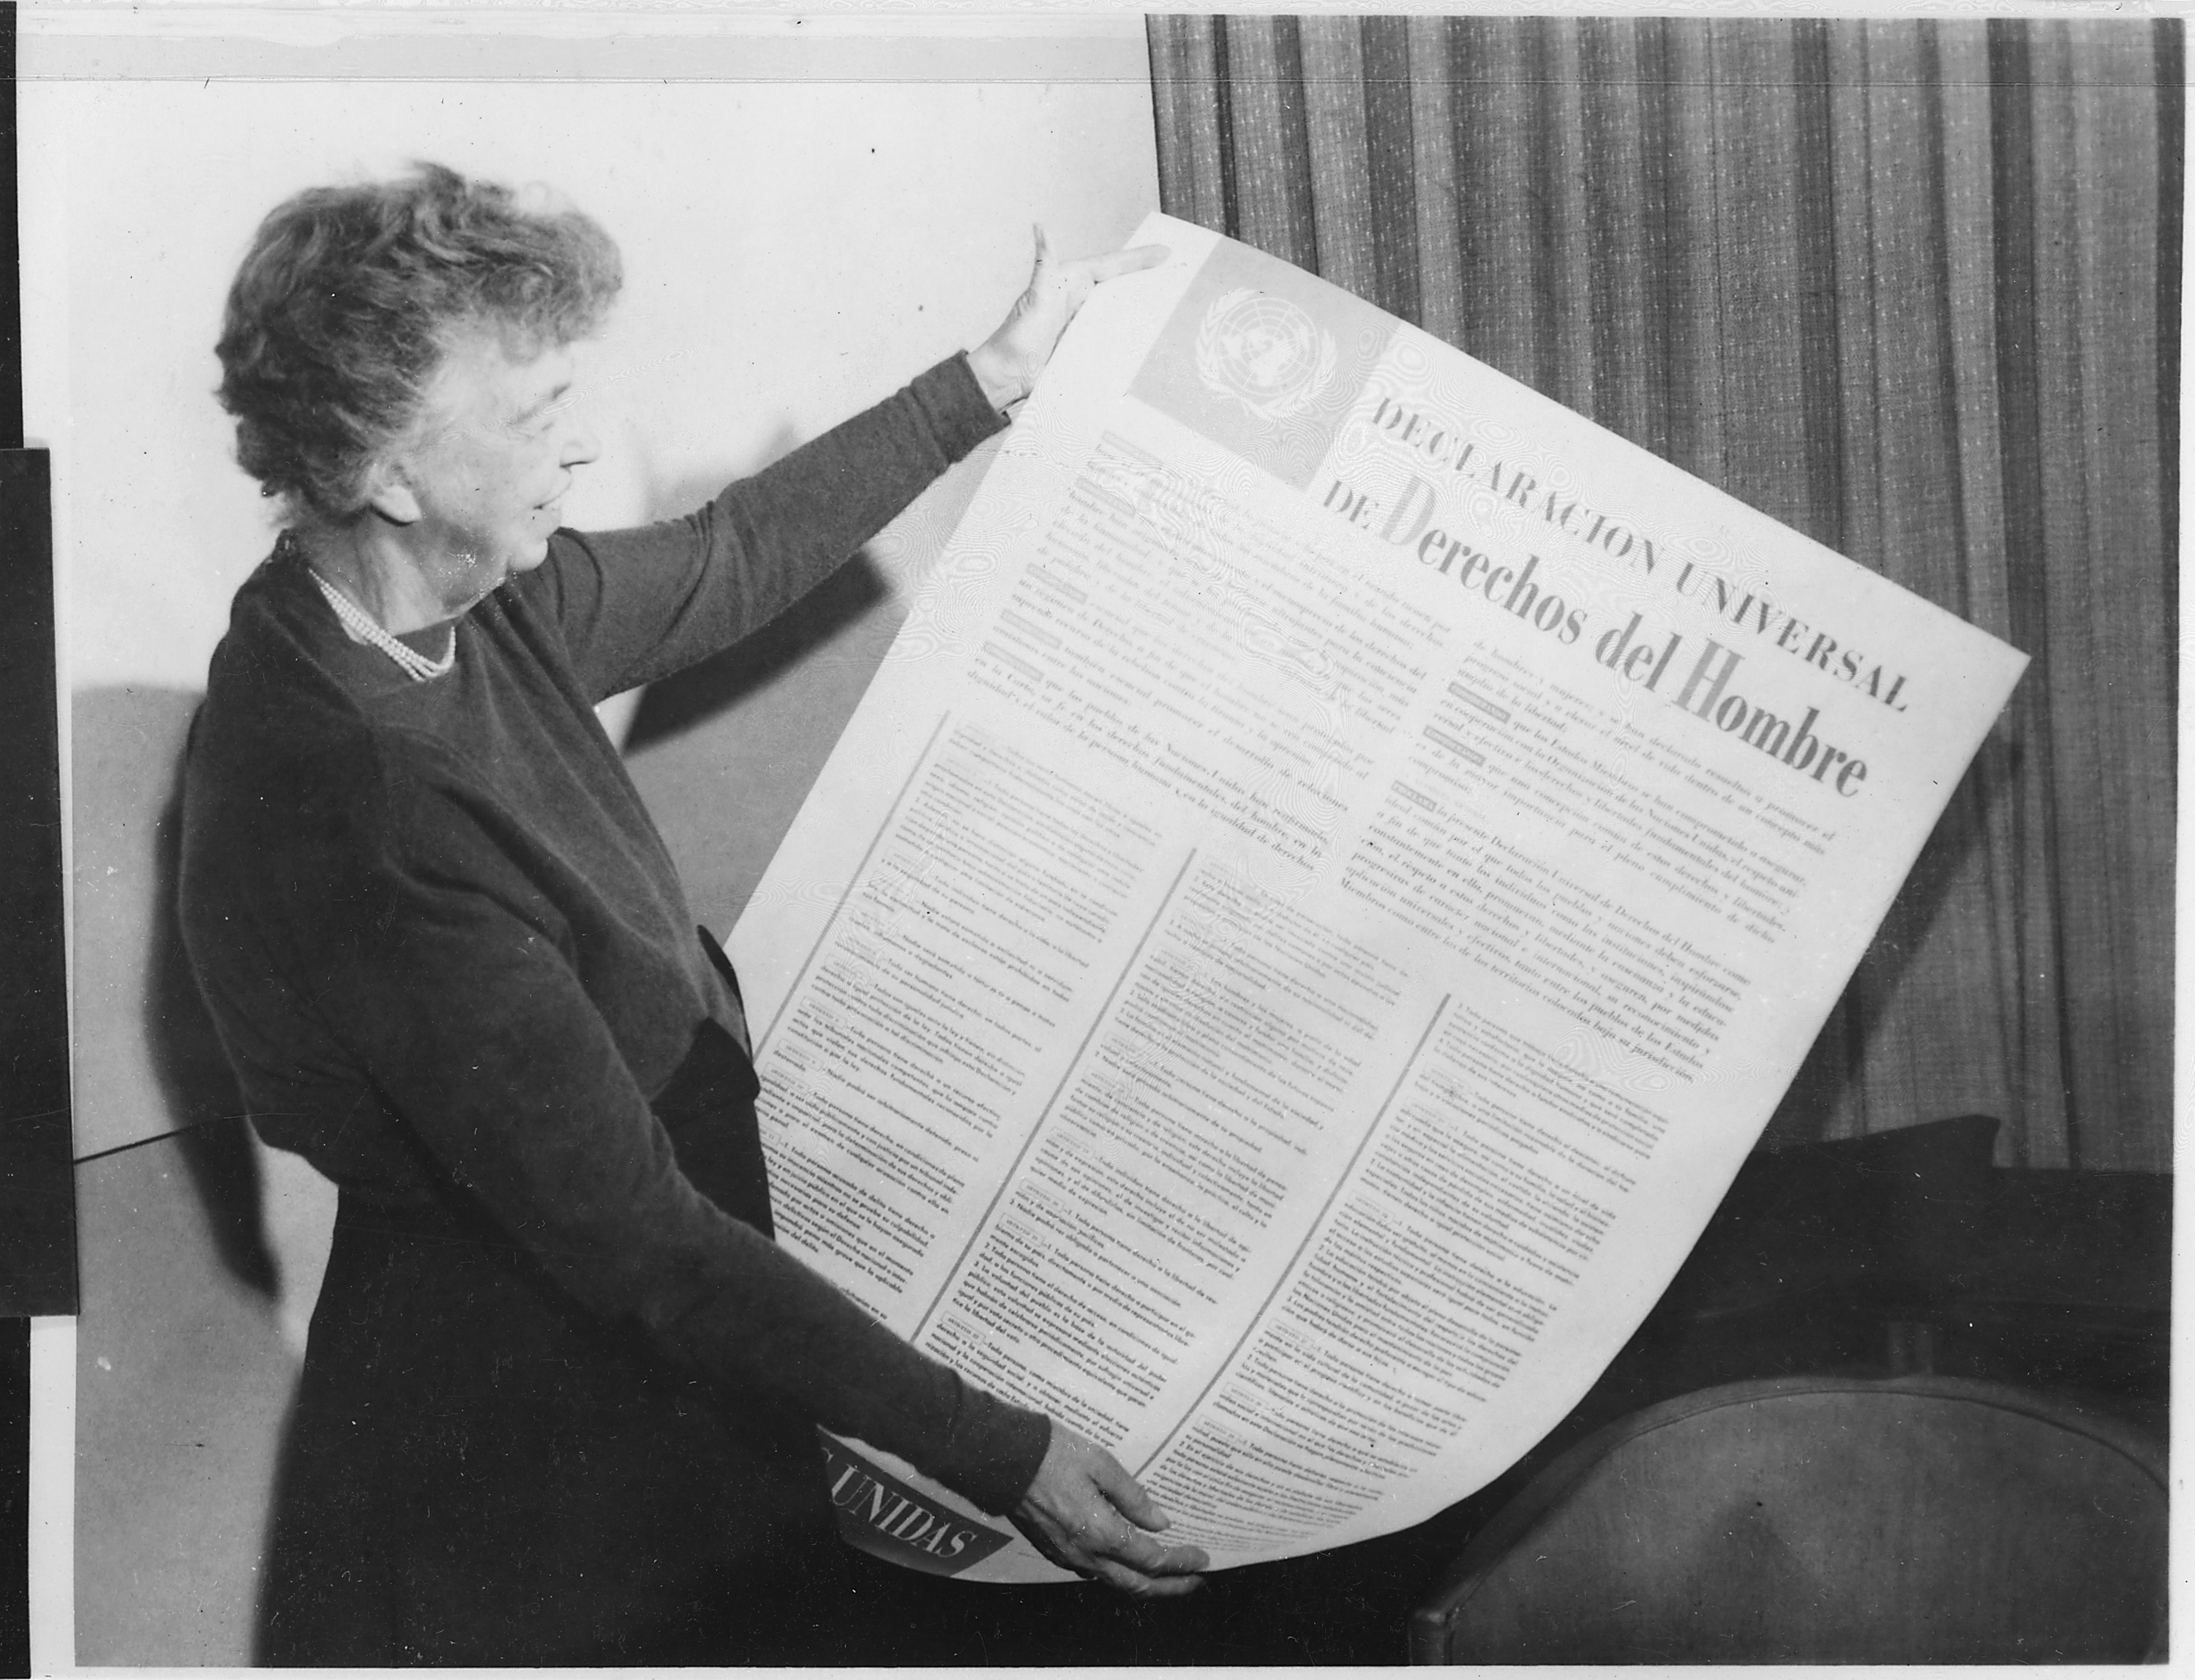
\includegraphics[width=70mm]{images/eleanor.jpg}
   \caption{エレノア・ルーズベルト}
 \end{figure}




\section{推薦図書}


\begin{itemize}
\item デイヴィッド・ウィナー『エリノア・ルーズベルト』、偕成社、1994。小学生向け偉人伝。エリノア・ルーズベルトの偉大さは日本では十分評価されていない。
\end{itemize}




 % \begin{wrapfigure}{r}{60mm}
 %   \begin{center}
 %     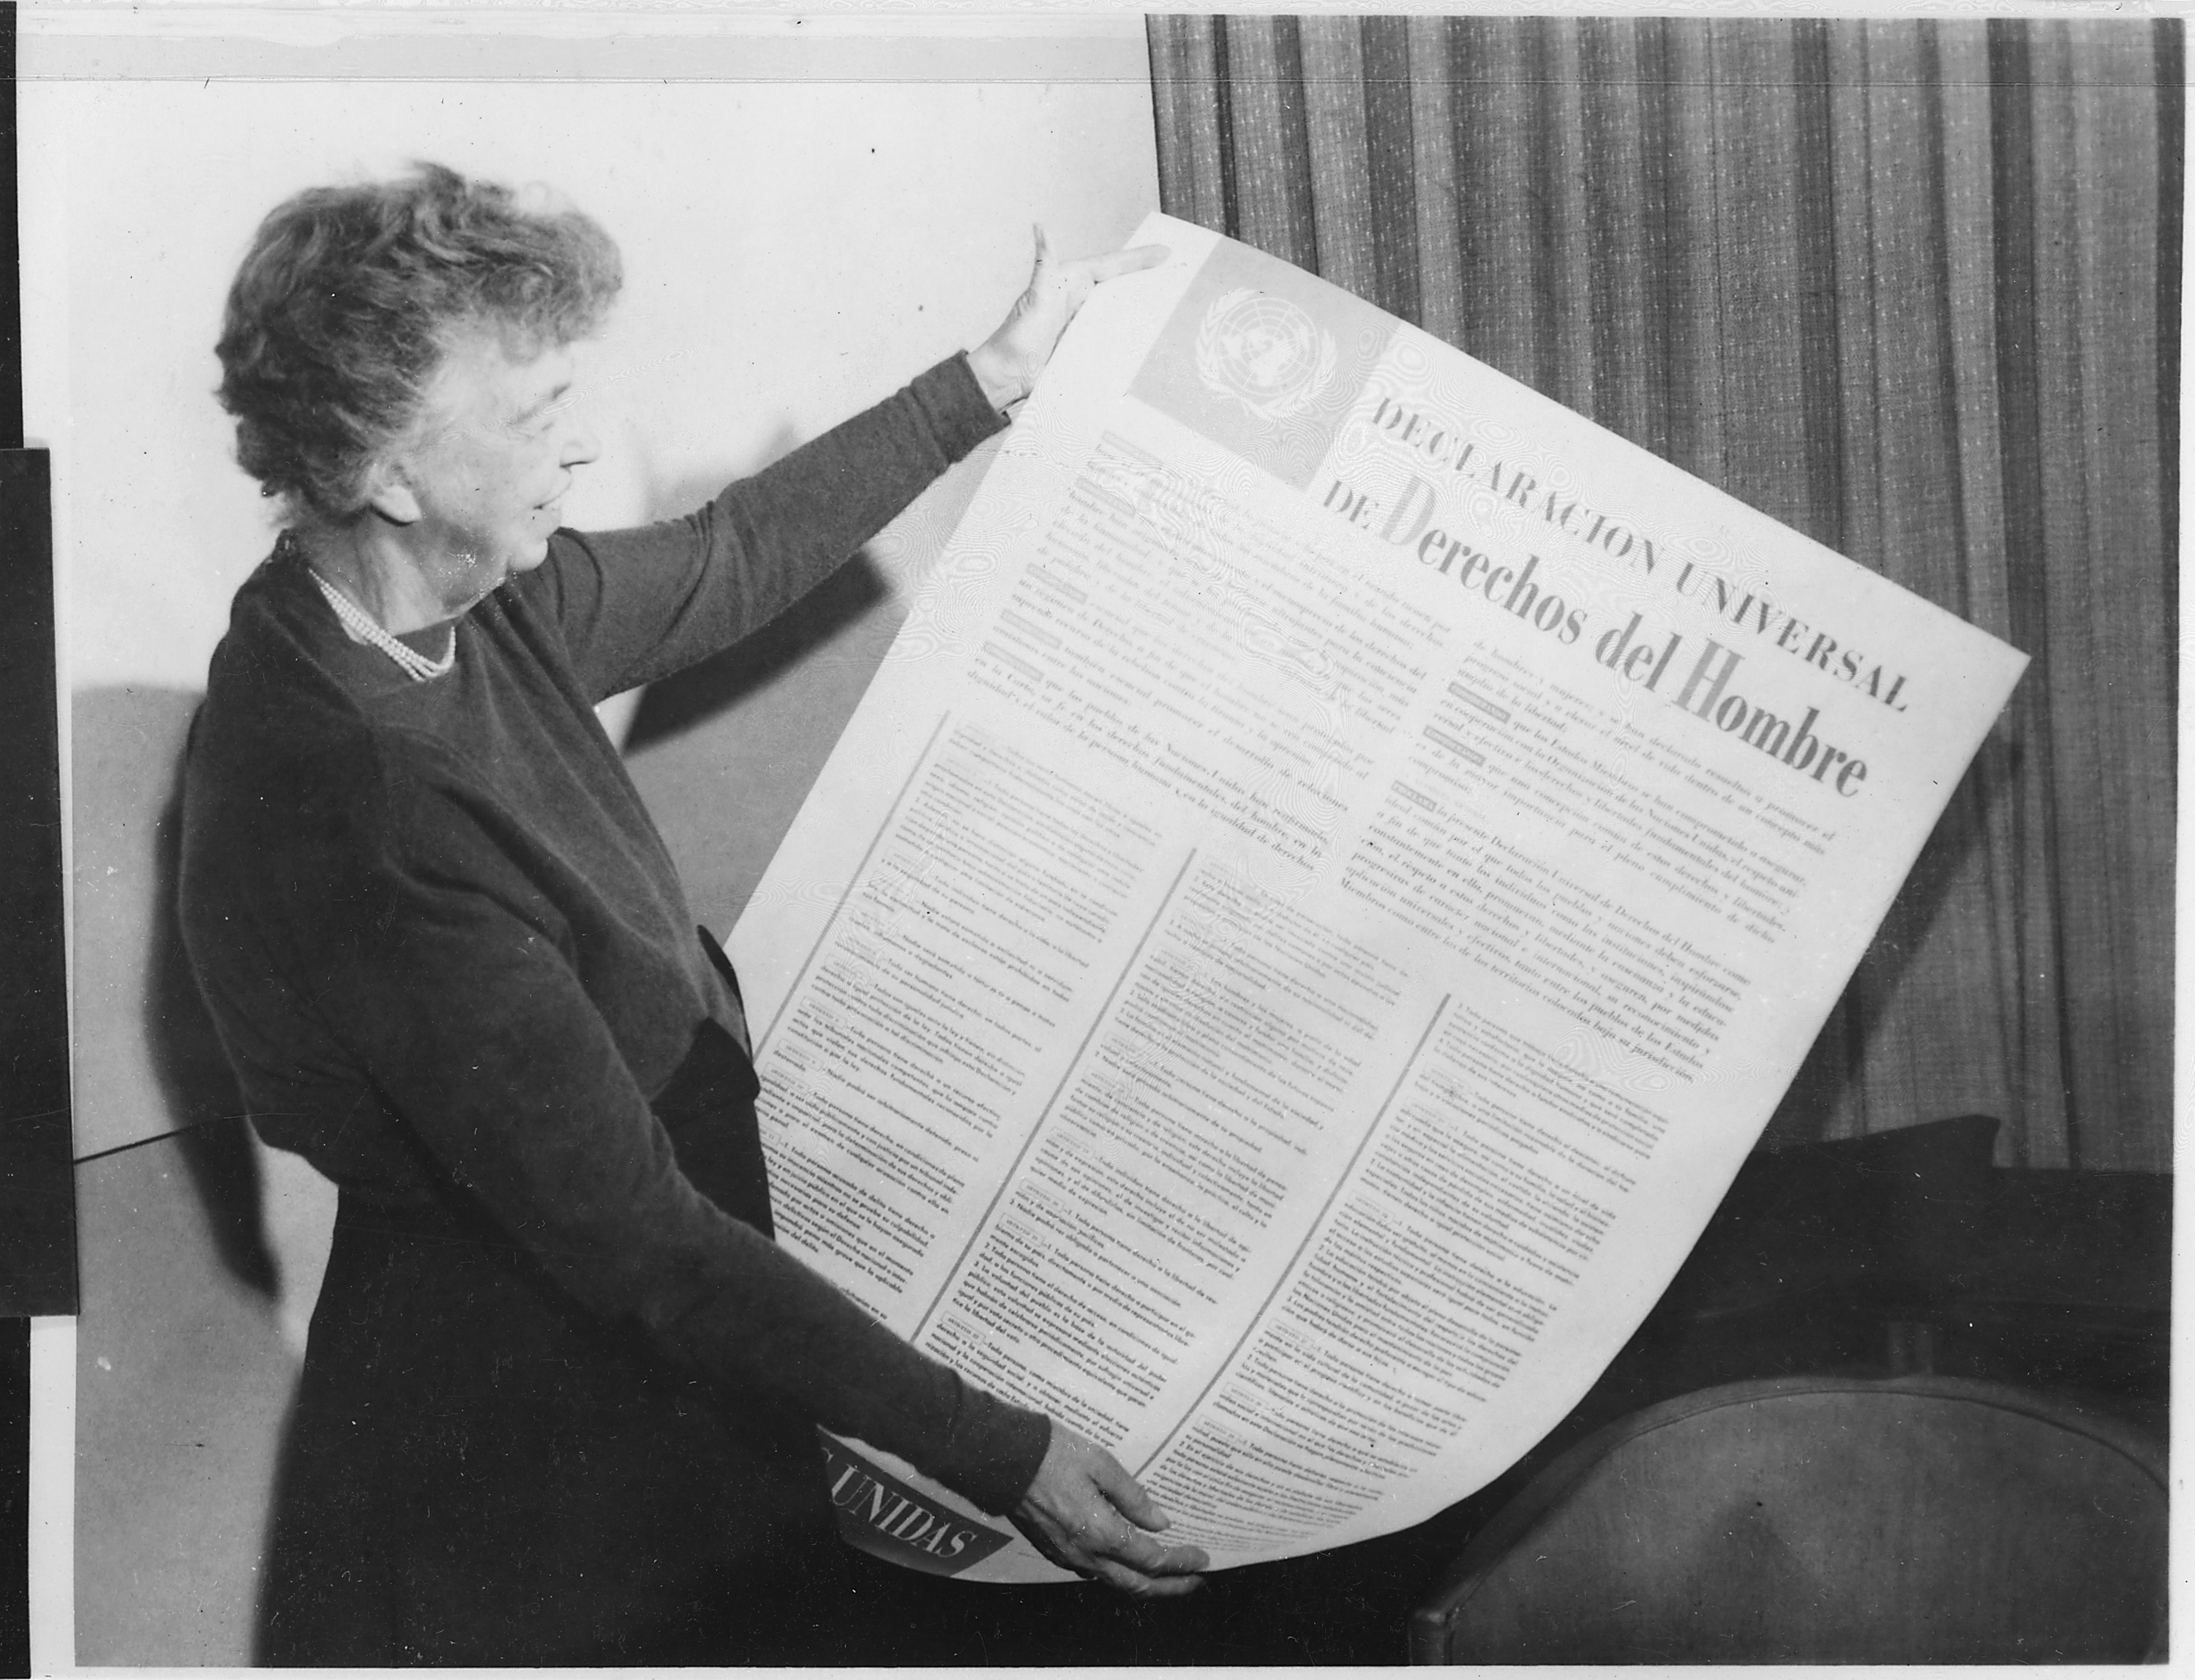
\includegraphics[width=70mm]{images/eleanor.jpg}
 %     \caption{エレノア・ルーズベルト} 
 %   \end{center}
 % \end{wrapfigure}




%%% Local Variables:
%%% mode: japanese-latex
%%% TeX-master: "main_gendai"
%%% coding: utf-8
%%% End:
